\section{Pentago}
\label{Pentago}
Pentago is a two-player abstract strategy game invented by Tomas Flodén. 
The company MindtwisterUSA \cite{MindTwisterUSA} has the rights of developing and commercializing the product in North America. %http://www.mindtwisterusa.com/product/classic-wood-pentago


\begin{wrapfigure}{r}{0.5\textwidth}
  \begin{center}
    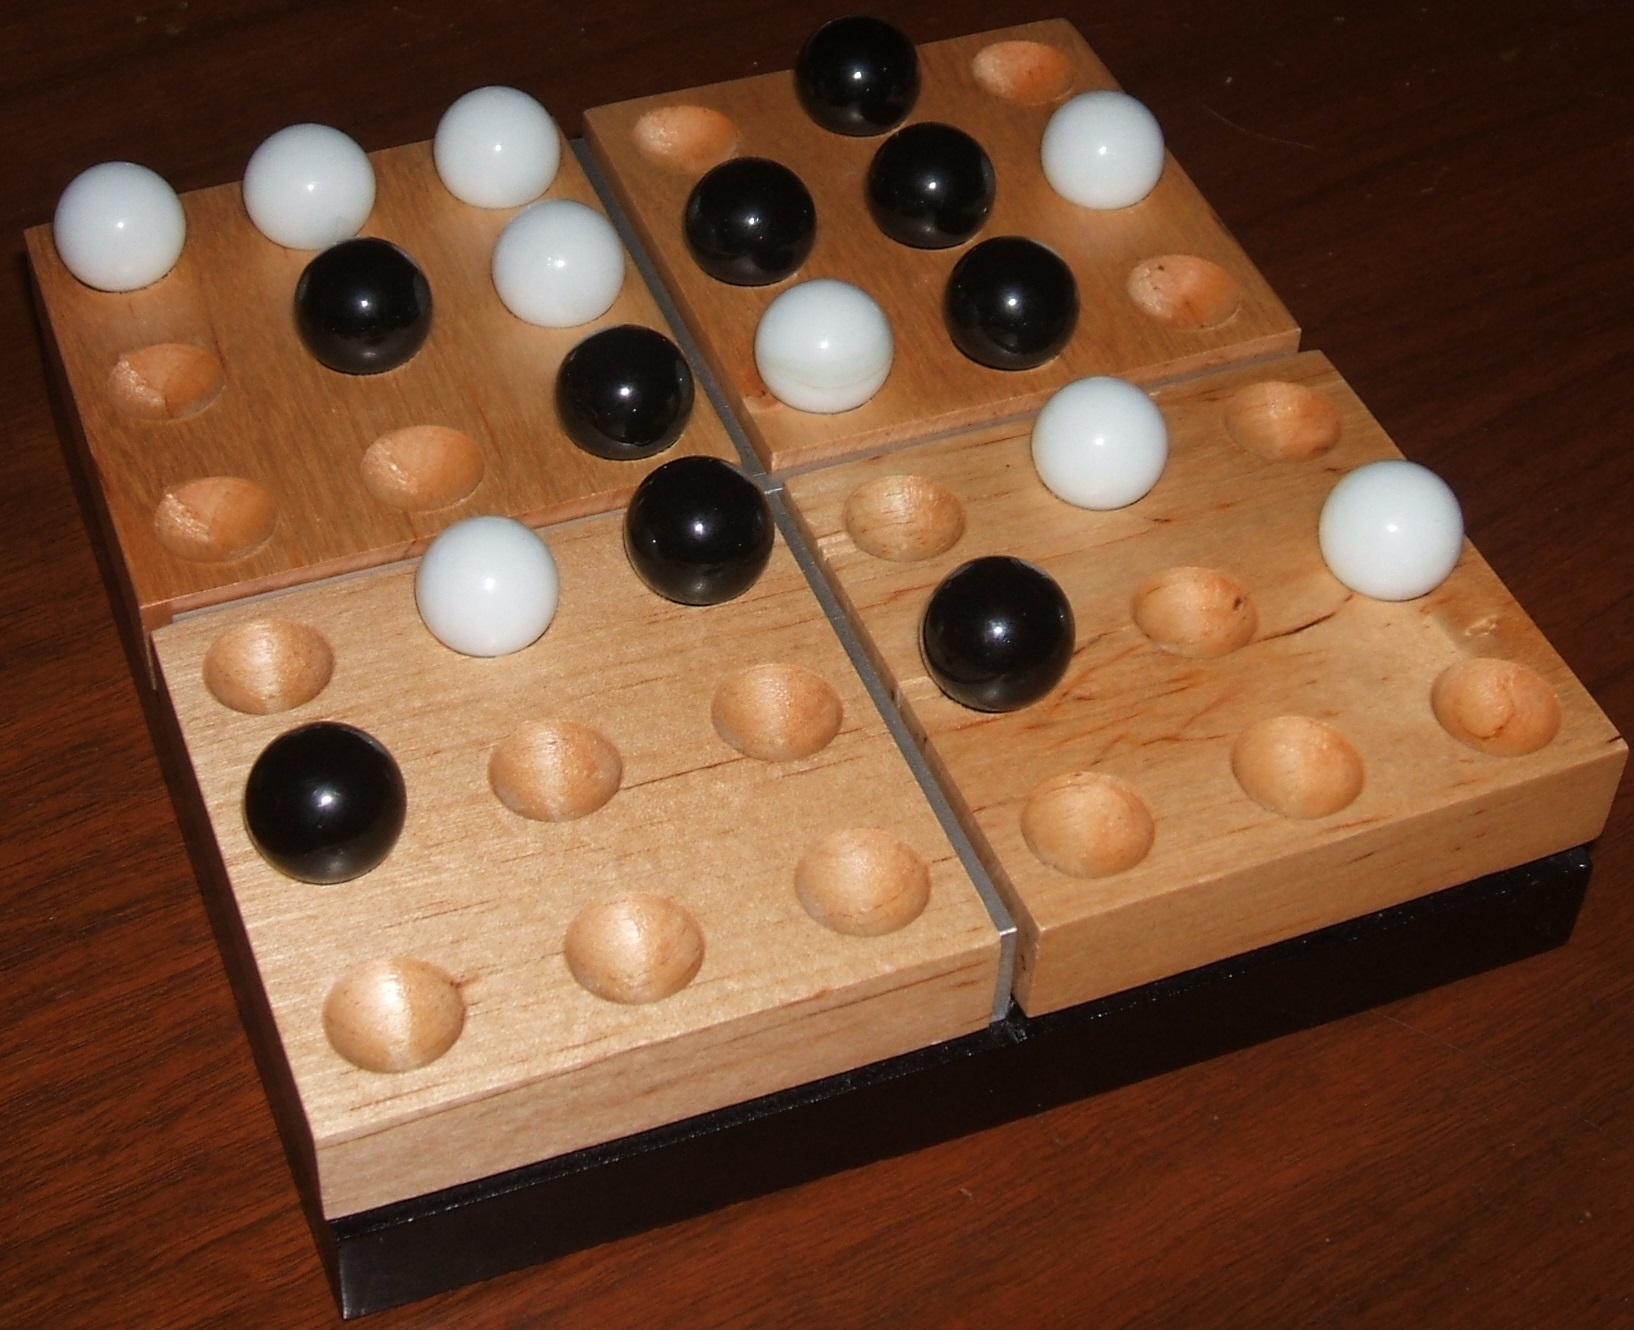
\includegraphics[width=0.48\textwidth]{Images/Pentago-Game-Winning-Position.jpg}
  \end{center}
  \caption{The pentago board}
  \label{fig:boardpic}
\end{wrapfigure}

\vspace{6pt}

Pentago is a two-player game invented by Tomas Flodén. 
The game is played on a 6×6 board divided into four 3×3 sub-boards (also called quadrants). 
Taking turns, the two players place a marble of their color onto an unoccupied space on the board, and then rotate one of the sub-boards by 90 degrees either clockwise or counter-clockwise. 
A player wins by getting five of its marbles in a vertical, horizontal or diagonal row. 
In figure \ref{fig:boardpic} player white wins by possessing a diagonal row. 
If all 36 spaces on the board are occupied without a row of five having formed then the game is a draw.
If multiple players achieve a row of five simultaneously, the game is a draw.
Also a multi-player version for 3 or 4 players has been developed and features a 9×9 board. 
This addition is called super-pentago. 
We plan to model pentago in a scalable fashion so that the board and player size can be defined on initialization.
